% !Mode::"TeX:UTF-8"

\documentclass[UTF8,a4paper,11pt]{article}
\usepackage{ctex}
\usepackage[top=1.54cm, bottom=1.54cm, left=2.30cm, right=2.30cm]{geometry}
\usepackage{graphicx}
\author{coorty}
\title{High Categorical Feature Process}

\begin{document}
\maketitle
现实生活中, 很多特征都是类型型特征. 比如衣服的颜色特征: 红, 绿, 蓝等; 城市的邮编; 对于前一种的颜色特征, 取值可能最多只有一二十个, 有时直接对其进行one-hot编码后就可以送入模型进行训练. 而对于邮编特征, 取值可能有上千个,这个时候再进行one-hot编码显然有点不合适, 会造成特征的维度很高, 而且效果可能也不会好. 这种特征被称为"高集势类别特征(High-cardinality categorical feature)". 

首先想到的是可不可以使用聚类的方式先对这些特征进行一个\textbf{聚类}, 如果取值总共有$N$个, 将其聚类到$K$个类中, 而且$K \ll N$, 就能达到降维的目的了. 但是这里有两个问题:

\begin{itemize}
\item 使用聚类的结果是代替类中的每个值, 会造成信息的丢失;
\item 如果类别型特征是非数值型的, 如何进行聚类? 	
\end{itemize}
	
可以使用\textbf{平均编码方法}(Mean Encoding)$^{[2]}$:

对于分类问题, 假设目标变量$y$总共有$K$类, 同时假设类别特征为$X$, 里面的所有unique值表示为$(X_1, X_2,...,X_n)$, 计算每个$X_i$取值下, 样本属于第$j$类的概率: 

$$ P(y=y_j|X=X_i) = \frac{Count(y=y_j, X=X_i)}{Count(X=X_i)} $$

这样, 每个$X_i$就能得到$K$个概率值, 使用这个$K$维的概率值来对类别$X_i$进行编码! 这是一种有监督的方式, 必须要知道每个样本对于的$Y$标签.

但是这种做法有一些缺点, 比如: (1) 计算的时候需要在已标记的样本上进行计算, 如果测试集上面有训练集上不存在的$X_i$, 如果得到它的编码? (2) 样本中每个类别$X_i$出现的次数有多,少之分, 主观上认为, 如果一个$X_i$出现的次数越多, 计算得到的后验概率就越可信, 出现次数越少越不可信. 如何修改公式以达到这两个目的? 可以引入一个权重:

$$ P=\lambda * P(\vec{y}) + (1-\lambda)*P(\vec{y}|X=X_i) $$

看看是否满足了上面的两个要求: (1) 如果出现了训练集中不存在的$X_i$, 则令$\lambda=0$(表示使用标记数据中每类样本出现的概率来进行编码); (2) $\lambda$ 不能是一个标量, 而应该是类别特征出现次数的一个函数, 假设$X_i$出现的次数为$m_i$次, 则其对于的$\lambda$为:

$$ \lambda (m=m_i) = \frac{1}{1+e^{(m_i-n)/f}} $$

由于$\lambda$的范围必须在0-1之间, 因此和sigmoid函数相似, 设计成$\frac{1}{1+e^{\Delta}}$的形式. 这里, $n$表示特征$X$中unique值的数量, $f$控制了函数的平滑性; 在$f$取不同的值时, $\lambda$函数如下所示:

\begin{figure}[htbp]
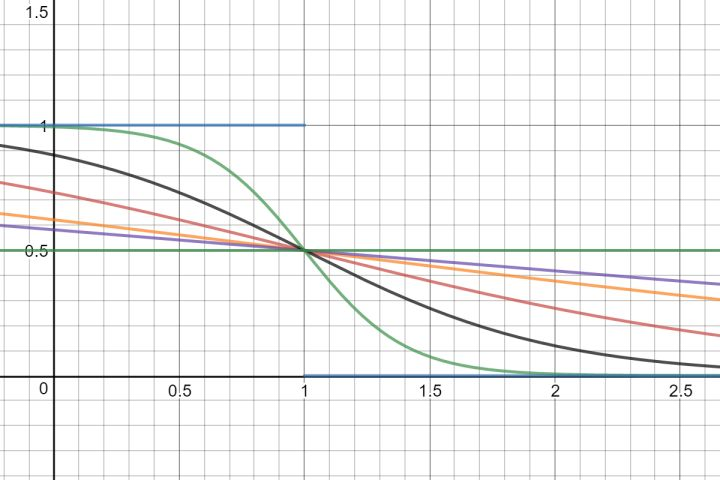
\includegraphics[width=0.7\textwidth]{images/lambda_function.jpg}
\centering
\caption{lambda function}	
\end{figure}

$\bullet$ 如果$m_i$很大, 表示类别$X_i$出现的次数很多, 则$\lambda$接近0, $1-\lambda$接近1, 表示充分信任后验概率(但是如果这样, 特征$X$的熵很小啊, 提供不了什么有用的信息, 应该直接丢弃这个特征).

$\bullet$ 如果$m_i$很小, 表示类别$X_i$出现的次数很少, 则$\lambda$接近1, $1-\lambda$接近0, 表示充分不信任后验概率(如果$m_i$等于0,则表示此类别特征在标记样本集中不存在啊, 因此没有后验概率).\\

\noindent \textbf{Note}: \\
(1) 实现时, 一般将标记样本分成$K$份, 利用$K-1$份进行fit, 对剩下的1份进行transform; 这个过程进行$K$次. 如果fit和transform的时候都使用全部的数据, 可能会造成模型过拟合(标记样本要分成训练和测试集, 如果对所有标记样本进行同时fit,transform, 则分成的训练和测试集之间就不是独立的了c).	
	
\begin{thebibliography}{9}
\bibitem{item1} Micci-Barreca D. A preprocessing scheme for high-cardinality categorical attributes in classification and prediction problems[J]. ACM SIGKDD Explorations Newsletter, 2001, 3(1): 27-32.
\bibitem{item2} Mean Encoding: A Preprocessing Scheme for High-Cardinality Categorical Features.
\bibitem{item3} https://zhuanlan.zhihu.com/p/26308272
\end{thebibliography}	

\end{document}


















